\section{Signal processing algorithm}\label{sec:processing}

\begin{wrapfigure}[12]{r}{.45\textwidth}
    \vspace{-\baselineskip}
    \centering
    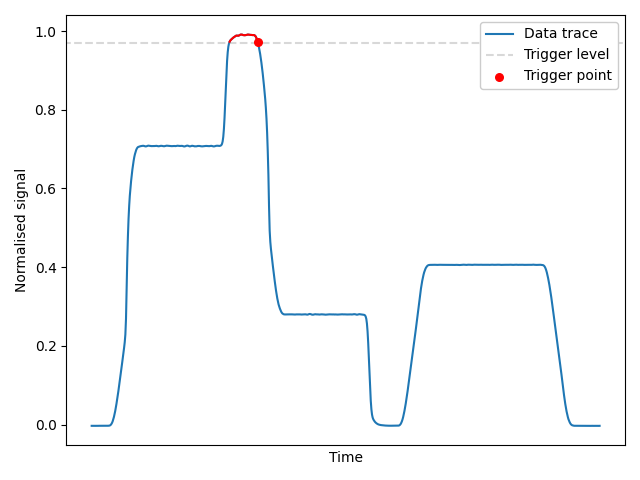
\includegraphics[width=.98\textwidth]{images/old_trace.png}
    \caption{Illustration of original algorithm}
    \label{fig:trace}
\end{wrapfigure}
In \cref{fig:trace} the signal of the photodiode is shown for one cycle of chopper 2, as described in \cref{sec:setup}. The five signal levels resulting from the different chopper configuration are clearly distinguishable. To process the signal, the following algorithm had been used. Initially, , for example at \qty{97}{\percent}, the software identifies trigger points when the signal falls below this level. Ideally, the triggering occurs at the falling edge of the total signal peak. The software utilizes these trigger points to determine the locations of the other signal levels and calculates the mean values of the flat levels. From these the software computes the sample reflectivity using the method outlined at the end of \cref{sec:setup}. 

However, this method exhibits some limitations when used for the automation for the setup. These limitations arise from the possibility to have multiple triggers in a single cycle, resulting in unusable measurement data and necessitating to manually adjusting the trigger and redoing the measurement. Such a manual process is counter productive to the aim of automation. To address this issue, it is essential to investigate the underlying causes.

\begin{wrapfigure}[9]{r}{.45\textwidth}
    \vspace{-2.5\baselineskip}
    \centering
    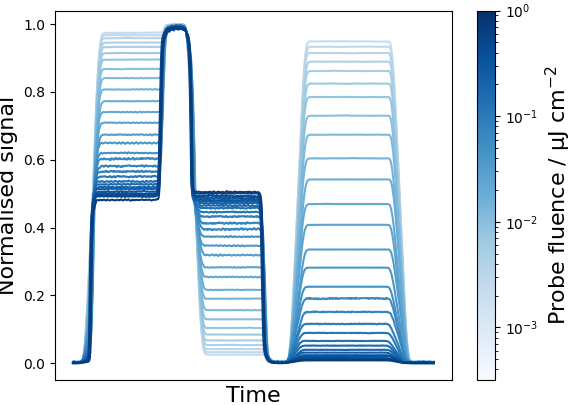
\includegraphics[width=.98\textwidth]{images/trace_complete.png}
    \caption{Signal for a fixed pump power and increasing amount of fluence. (NEED TO ADD AXIS LABEL TO IMAGE)}
    \label{fig:complete}
\end{wrapfigure}
For one, there is the nature of the measured signal. Since all levels are measured simultaneously and with the same detector, their signal strength are in relation to each other. As a result, high variations in signal levels occur during a measurement, as illustrated in \cref{fig:complete}. Since measurements are conducted for different pump powers, the influence of the PL has to be taken into account. Initially, at low probe fluences, the PL signal dominates, requiring to set a trigger level to ensure triggering on the total level rather than the PL level. 

\begin{wrapfigure}{r}{.45\textwidth}
    \vspace{-\baselineskip}
    \centering
    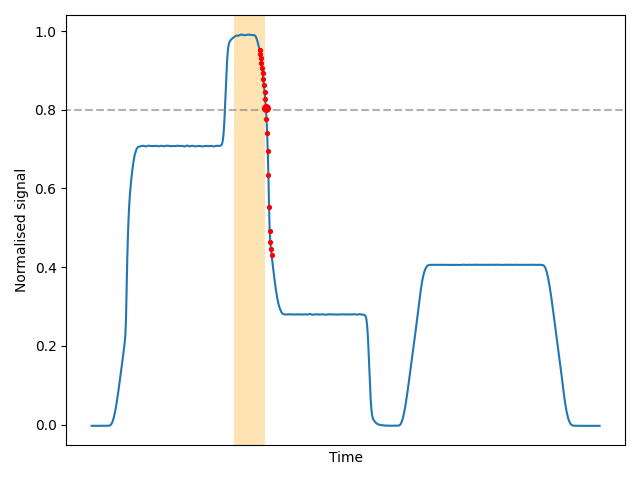
\includegraphics[width=.98\textwidth]{images/corrected_signal.png}
    \caption{Illustration of improved algorithm}
    \label{fig:corrected}
\end{wrapfigure}
To address these mistriggering cases, the following method has been implement which has also been illustrated in \cref{fig:corrected}. By utilizing the approach described above but with a lower triggering value of \qty{80}{\percent}, avoids triggering on a noisy total level but allows for triggering on both the total peak and the PL peak. Additionally, this introduces the risk of triggering on a noisy signal level that may lay close to the trigger level during a measurement. To address this, neighbouring points (small red dots in \cref{fig:corrected}) of the triggers are examined and ensuring that the signal level is descending. Finally, we verify that we are on the total peak by requiring that a maximum value of the signal is in close proximity (orange shaded area in \cref{fig:corrected}) to the trigger point.

Using this method allowed for the automated measurement process to successfully be finished.
Resulting in a decease of 5\% in measurement time and the fully autonomous measuring of data.